Procedemos a preparar una máquina virtual con Ubuntu 22.04, el cual le instalamos el volatility según en el siguiente enlace:

\begin{itemize}
    \item https://www.youtube.com/watch?v=5-2-ORNC8CA
\end{itemize}

A continuación procedemos a buscar el perfil con volatility con el comando imageinfo.

\begin{figure}[htp]
    \centering
    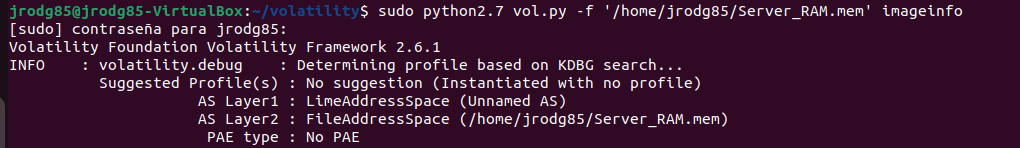
\includegraphics[width=1.0\textwidth]{imagenes/009-captura-imgeinfo.png}
    \caption{captura imageinfo}
    \label{captura imageinfo.}
\end{figure}

Como se puede observar en la imagen anterior, no hemos llegado a encontrar un perfil concreto con imageinfo, eso se debe a que el perfil creado no es el que se encuentra dentro de las conocidas en la base de datos de volatility. Por ello procedemos a buscar dentor de la memoria RAM un string que tenga la cadena de texto "linux version". para ello ejecutamos el comando $strings Server_{RAM}.mem \mid grep -Ei linux version \mid uniq$.

\begin{figure}[htp]
    \centering
    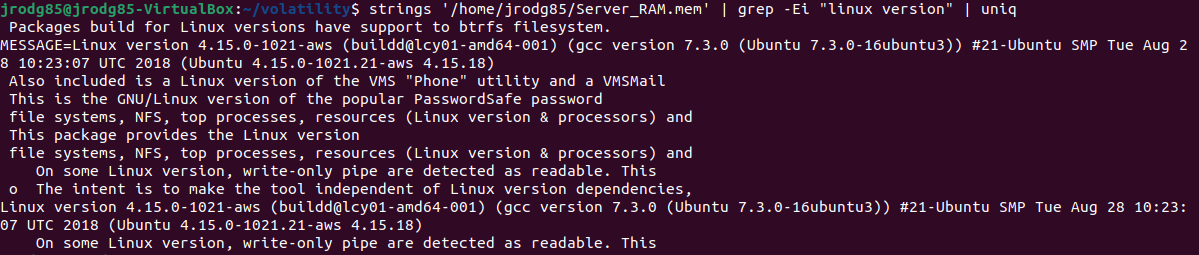
\includegraphics[width=1.0\textwidth]{imagenes/010-buscar-strings-linux-verison.png}
    \caption{captura imageinfo}
    \label{captura linux version.}
\end{figure}


Podemos observar en la imagen anterior que el sistema operativo que utiliza en nuestro caso es un sistema operativo Linux para Amazon Web Service, concretamente el sistema operativo es el \textbf{4.15.0-1021.21-aws 4.15.18}. Esta version de Linux, es muy usada para las instancias de Amazon Web Services.

Como no tenemos el perfil cargado dentro de volatility, nos va a tocar hacer la tarea de cargar un perfil de este Sistema operativo para poder seguir ejecutando la aplicación volatility.

Buscando en google \textbf{linux version 4.15.0-1021.21-aws volatility}, nos encontramos solo un enlace en internet, el cual es https://lists.ubuntu.com/archives/bionic-changes/2018-August/016183.html, con ello nos encontrábamos con algo que ya se intuía previamente, y es que la versión del server de AWS, es basada en un ubuntu 18.04, ya que la fecha que indica 4.15.18 es una fecha en tipo "d.mm.aa".



